\documentclass[10pt]{beamer}
\usetheme[
%%% options passed to the outer theme
%    hidetitle,           % hide the (short) title in the sidebar
%    hideauthor,          % hide the (short) author in the sidebar
%    hideinstitute,       % hide the (short) institute in the bottom of the sidebar
%    shownavsym,          % show the navigation symbols
%    width=2cm,           % width of the sidebar (default is 2 cm)
%    hideothersubsections,% hide all subsections but the subsections in the current section
%    hideallsubsections,  % hide all subsections
    left               % right of left position of sidebar (default is right)
%%% options passed to the color theme
%    lightheaderbg,       % use a light header background
  ]{AAUsidebar}

% If you want to change the colors of the various elements in the theme, edit and uncomment the following lines
% Change the bar and sidebar colors:
%\setbeamercolor{AAUsidebar}{fg=red!20,bg=red}
%\setbeamercolor{sidebar}{bg=red!20}
% Change the color of the structural elements:
%\setbeamercolor{structure}{fg=red}
% Change the frame title text color:
%\setbeamercolor{frametitle}{fg=blue}
% Change the normal text color background:
%\setbeamercolor{normal text}{bg=gray!10}
% ... and you can of course change a lot more - see the beamer user manual.


\usepackage[utf8]{inputenc}
\usepackage[english]{babel}
\usepackage[T1]{fontenc}
% Or whatever. Note that the encoding and the font should match. If T1
% does not look nice, try deleting the line with the fontenc.
\usepackage{helvet}
\usepackage{tikz}
\usetikzlibrary{shapes,shapes.geometric, arrows,positioning,calc}
\tikzset{
	block/.style = {draw, fill=white, rectangle, minimum height=3em, minimum width=3em},
	tmp/.style  = {coordinate}, 
	sum/.style= {draw, fill=white, circle, node distance=1cm},
	input/.style = {coordinate},
	output/.style= {coordinate},
	pinstyle/.style = {pin edge={to-,thin,black}
	}
}

% colored hyperlinks
\newcommand{\chref}[2]{%
  \href{#1}{{\usebeamercolor[bg]{AAUsidebar}#2}}%
}

\title[Modelling and Networked Control of Water Distribution Networks]% optional, use only with long paper titles
{Modelling and Networked Control of Water Distribution Networks}

% \subtitle{}  % could also be a conference name

\date{\today}

\author[CA733] % optional, use only with lots of authors
{
  CA733
}
% - Give the names in the same order as they appear in the paper.
% - Use the \inst{?} command only if the authors have different
%   affiliation. See the beamer manual for an example

\institute[
%  {\includegraphics[scale=0.2]{aau_segl}}\\ %insert a company, department or university logo
  Control and Automation\\
  Aalborg University\\
  Denmark
] % optional - is placed in the bottom of the sidebar on every slide
{% is placed on the title page
  Control and Automation, Group 733\\
  Aalborg University\\
  Denmark
  
  %there must be an empty line above this line - otherwise some unwanted space is added between the university and the country (I do not know why;( )
}


% specify a logo on the titlepage (you can specify additional logos an include them in 
% institute command below
\pgfdeclareimage[height=1.5cm]{titlepagelogo}{AAUgraphics/aau_logo_new} % placed on the title page
%\pgfdeclareimage[height=1.5cm]{titlepagelogo2}{graphics/aau_logo_new} % placed on the title page
\titlegraphic{% is placed on the bottom of the title page
  \pgfuseimage{titlepagelogo}
%  \hspace{1cm}\pgfuseimage{titlepagelogo2}
}


\begin{document}
% the titlepage
{\aauwavesbg%
\begin{frame}[plain,noframenumbering] % the plain option removes the sidebar and header from the title page
  \titlepage
\end{frame}}
%%%%%%%%%%%%%%%%

% TOC
\begin{frame}{Agenda}{}
\tableofcontents
\end{frame}
%%%%%%%%%%%%%%%%

\section{Introduction}


% motivation for creating this theme
\begin{frame}{Introduction}{Introduction to Water Distribution Networks}
\begin{itemize}
	\item Critical societal infrastructure, responsible for the provision of water to both domestic and industrial consumers. 
	\item Network pressure must be controlled.
	\begin{itemize}
		\item Underpressure $\rightarrow$ insufficient service pressure $\rightarrow$ dissatisfied end users.
		\item Overpressure $\rightarrow$ component failure $\rightarrow$ repair costs, supply intermittency, etc.
	\end{itemize}
	\item Network pressure tied to level in Elevated Water Reservoir(s) (EWR) $\rightarrow$ level control is key!
	\item Other key components are pumps, valves, and pipes.
\end{itemize}
\end{frame}
\begin{frame}{Introduction}{Test Water Distribution Network Layout}
\begin{block}{}
	We analyse a small-scale test WDN with the following layout:
\end{block}

\begin{figure}[h]
	\centering
	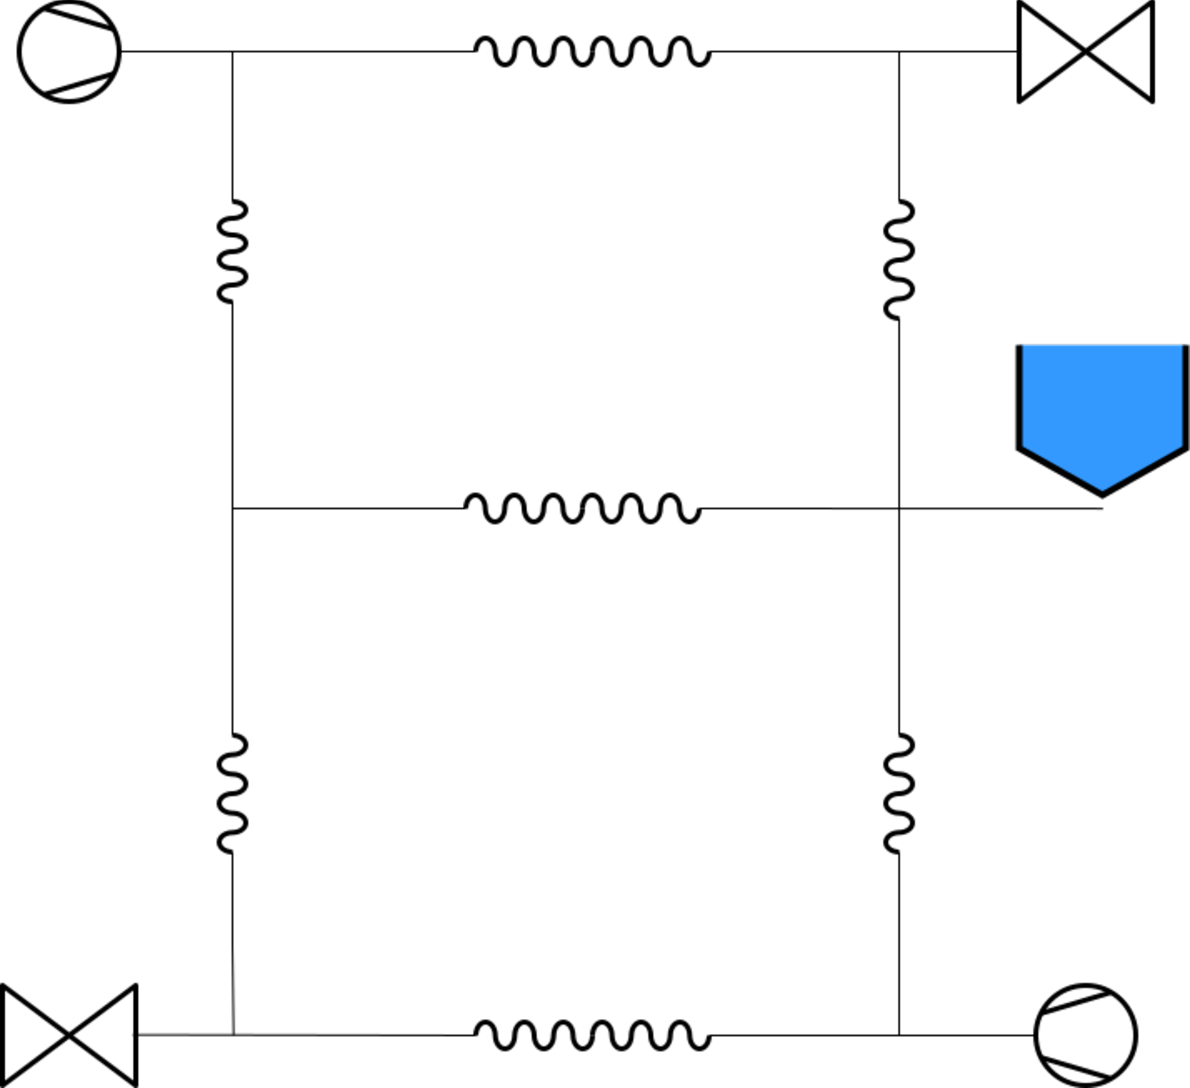
\includegraphics[width=0.5\linewidth]{Graphics/WDNModel.pdf}
	\label{fig:WDNModel}
	\begin{block}{}
		Larger WDNs are typically not amenable to first-principles modelling.
	\end{block}
\end{figure}

\end{frame}
%%%%%%%%%%%%%%%%

% ======================================================================
% Inputs for topics here!

\section{Modelling of WDN}

\begin{frame}{Modelling of WDN}
	divided in two sections..?
\end{frame}
\section{Fast Dynamics and Graph theory}
%\input{Topics/XX/XX}
%
\section{Slow Dynamics and Linearisation}
\subsubsection{Slow Dynamics}

\begin{frame}{Modelling of Water Distribution Networks}{Slow Dynamics}
	\begin{columns}
		\begin{column}{.5\textwidth}
			\begin{itemize}
				\item Fundamentals
				\begin{equation*}
					p \propto h 
				\end{equation*}
				\begin{equation*}
					\dot{V} = q
				\end{equation*}
				\item Assume constant cross sectional area A
				\begin{equation*}
					V \propto h \implies V \propto p 
				\end{equation*}
				\begin{equation*}
					\dot{p} \propto \dot{V} \wedge \dot{V} = q \implies \dot{p} \propto q
				\end{equation*}
				\item We arrive at
				\begin{equation*}
					\dot{p} = -\tau q \text{,  where}
				\end{equation*}	
				\begin{equation*}
					\tau = \rho g \frac{1}{A}
				\end{equation*}	
			\end{itemize}
		\end{column}
		\begin{column}{.5\textwidth}\raggedleft
			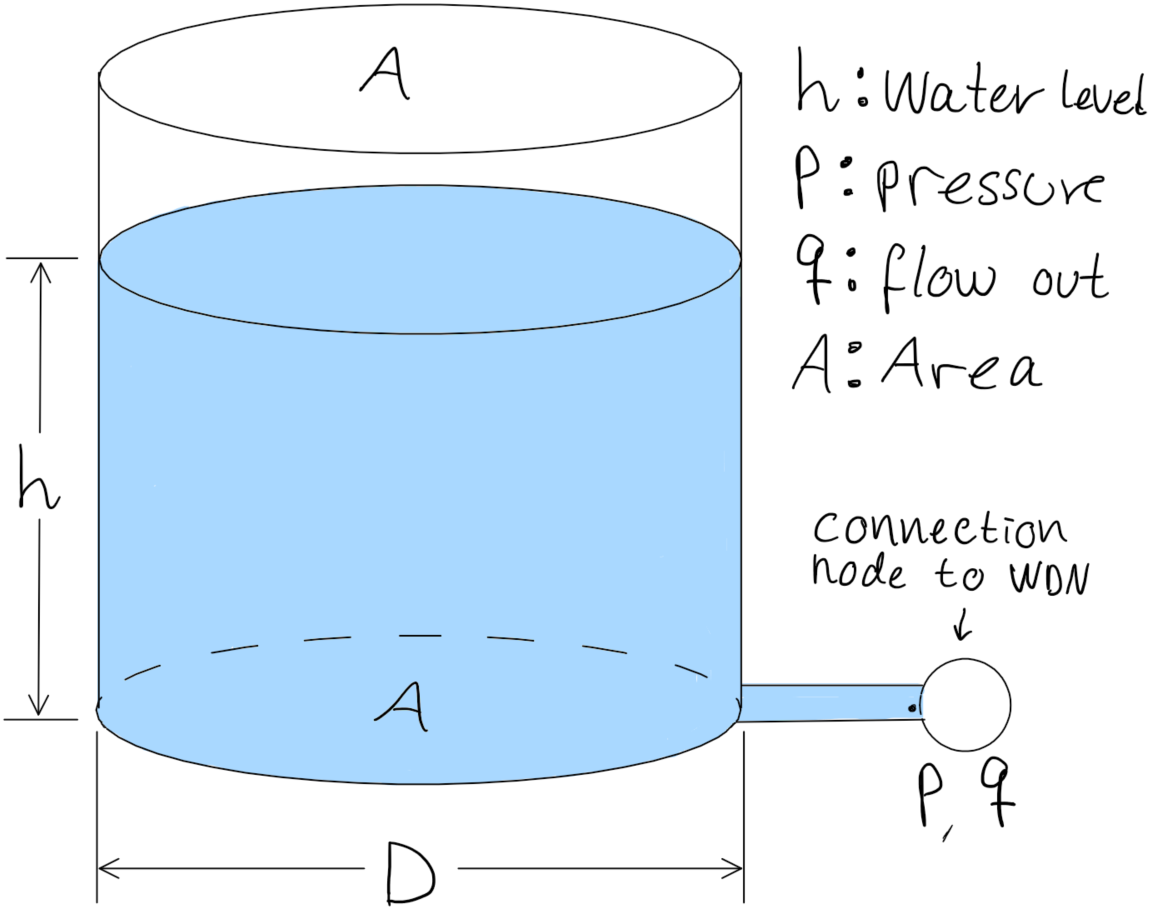
\includegraphics[width=1\linewidth]{Topics/SlowDynamicsLinearisation/Graphics/Tank_sketch.png}
		\end{column}
	\end{columns}
\end{frame}

\begin{frame}{Modelling of Water Distribution Network}{State-space Formulation of Slow Dynamics}
	\begin{figure}[h!]
		\centering
		\resizebox{\columnwidth}{!}{
				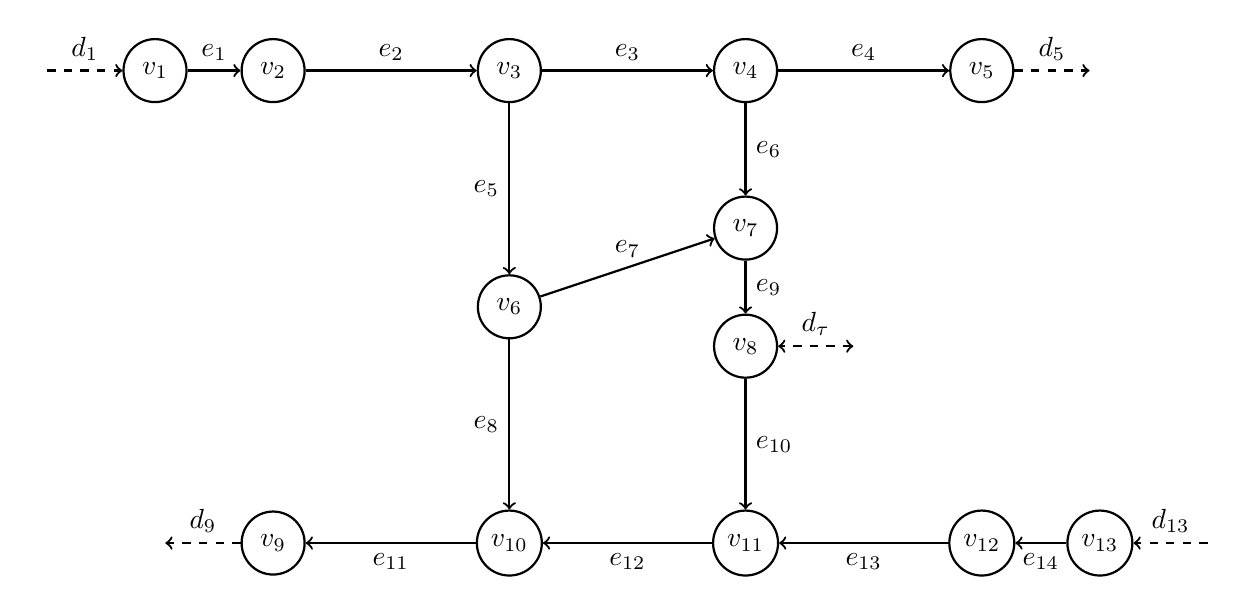
\begin{tikzpicture}[node distance=30mm, thick, main/.style = {draw,circle,minimum size=0.8cm}] 
		\node (1)  {};
		\node[main] (2) [node distance={15mm},right of=1] {$v_1$}; 
		\node[main] (3) [node distance={1.5cm},right of=2] {$v_2$};
		\node[main] (4) [right of=3] {$v_3$};
		\node[main] (5) [right of=4] {$v_4$};
		\node[main] (6) [right of=5] {$v_5$};
		\node (7) [node distance={15mm},right of=6] {};
		%Create 3 (4) nodes in middle part of graph
		\node[main] (8) [below of=4] {$ v_6 $};
		\node[main] (9) [node distance={20mm},below of=5] {$ v_7 $};
		\node[main] (11) [node distance={15mm},below of=9] {$ v_8 $};
		\node (10) [node distance={15mm},right of=11] {};
		%First 5 (7) nodes in bottom part of graph
		\node[main] (12) [below of=8] {$ v_{10} $};
		\node[main] (13) [left of=12] {$ v_9 $};
		\node(14) [node distance={15mm},left of=13] {};
		\node[main] (15) [right of=12] {$ v_{11} $};
		\node[main] (16) [right of=15] {$ v_{12} $};
		\node[main] (17) [node distance={1.5cm},right of=16] {$ v_{13} $};
		\node(18) [node distance={15mm},right of=17] {};
		
		%Edges with direction
		\path [->] (2) edge node[above] {$e_{1}$} (3); 	%Edge v1 -> v2
		\path [->] (3) edge node[above] {$e_{2}$} (4); 	%Edge v2 -> v3
		\path [->] (4) edge node[above] {$e_{3}$} (5); 	%Edge v3 -> v4
		\path [->] (5) edge node[above] {$e_{4}$} (6); 	%Edge v4 -> v5
		
		\path [->] (4) edge node[left] {$e_{5}$} (8); 	%Edge v3 -> v6
		\path [->] (5) edge node[right] {$e_{6}$} (9); 	%Edge v4 -> v7
		\path [->] (8) edge node[above] {$e_{7}$} (9); 	%Edge v6 -> v7
		\path [->] (8) edge node[left] {$e_{8}$} (12); 	%Edge v6 -> v10
		\path [->] (9) edge node[right] {$e_{9}$} (11); 	%Edge v7 -> v8
		\path [->] (11) edge node[right] {$e_{10}$} (15);	 %Edge v8 -> v11
		
		
		\path [->] (12) edge node[below] {$e_{11}$} (13); %Edge v10 -> v9
		\path [->] (15) edge node[below] {$e_{12}$} (12); %Edge v11 -> v10
		\path [->] (16) edge node[below] {$e_{13}$} (15); %Edge v12 -> v11
		\path [->] (17) edge node[below] {$e_{14}$} (16); %Edge v13 -> v12
		
		%External flows
		\draw[->,dashed,] (1) -- node[above] {$d_1$} (2); %Create d1
		\draw[->,dashed,] (6) -- node[above] {$d_5$} (7); %Create d5
		\draw[->,dashed,] (13) -- node[above] {$d_9$} (14); %Create d13
		\draw[->,dashed,] (18) -- node[above] {$d_{13}$} (17); %Create d13
		\draw[<->,dashed,] (10) -- node[above] {$d_\tau$} (11); %Create d_tau
	\end{tikzpicture} }
		\label{fig:tikzWDNGraph}
	\end{figure}  
	In context of WDN we now consider flows to and from network as external demands $ d_i $
\end{frame}

\begin{frame}{Modelling of Water Distribution Networks}{State-space Formulation of Slow Dynamics}
	Mass conservation holds, and such
	\begin{equation*}
		d_n = -\sum_{i=1}^{n-1}d_i \implies d_\tau = - (d_p + d_c)
	\end{equation*}
	\begin{equation*}
		\dot{p} = -\tau d_\tau = \tau (d_p + d_c)
	\end{equation*}	
	When discretised by forward Euler:
	\begin{equation*}
		p_\tau(k+1) = p_\tau(k) - \tau d_\tau(k) t_s = p_\tau(k) + \tau(d_p(k) + d_c(k)) t_s
	\end{equation*}
	Which corresponds to a discrete, linear state-space model:
	\begin{equation}
		p_\tau(k+1) = Ap_\tau(k) + B_pd_p(k) + B_cd_c(k)
	\end{equation}
	\begin{equation*}
		d_p = \begin{bmatrix}
			d_1 \\ d_{13}
		\end{bmatrix},
		d_c = \begin{bmatrix}
			d_5 \\ d_9
		\end{bmatrix},
		B_p = B_c = t_s  \begin{bmatrix}
			\tau & \tau
		\end{bmatrix},
		A = 1
	\end{equation*}
\end{frame}


\subsubsection{Linearisation}
\begin{frame}{Modelling of Water Distribution Networks}{Linearisation}
	\begin{columns}
		\begin{column}{.4\textwidth}
			\begin{itemize}
				\item Fast dynamics are non-linear
				\item Linearisation required
			\end{itemize}
			In near vicinity of linearisation point $ x_0 $,
			\begin{equation*}
				\dot{x} \approx f(x_0) + \nabla f\bigg\rvert_{x_0} (x-x_0)
			\end{equation*}
			Linearising around equilibrium point preferred
		\end{column}
		\begin{column}{.6\textwidth}\raggedleft
			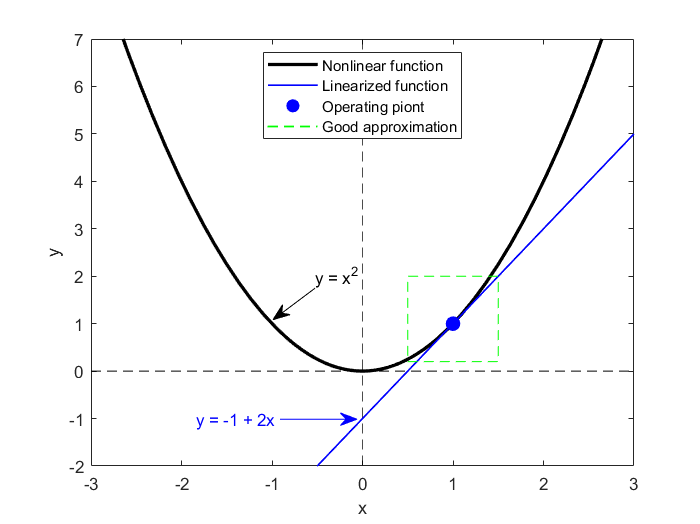
\includegraphics[width=1\linewidth]{Topics/SlowDynamicsLinearisation/Graphics/Linearisation_pic.png}
		\end{column}
	\end{columns}
\end{frame}

\begin{frame}{Modelling of Water Distribution Networks}{Linearisation}
%	Fast dynamics are non linear - linearisation is needed.\\
%	In near vicinity of linearisation point $ x_0 $,
%	\begin{equation*}
%		\dot{x} \approx f(x_0) + \nabla f\bigg\rvert_{x_0} (x-x_0)
%	\end{equation*}
	Recalling the fast dynamics differential equation is given as
	\begin{equation}\label{eq:NonLinearModelSimplified}
		\begin{split}
			\dot{q}_n &=  -\mathcal{P}\Phi\Big(\lambda(q_n)+\mu(q_n,\Theta)+\alpha(q_n,\omega)\Big) +\\ &\mathcal{P}\Big(\Psi(\bar{h}-\mathbf{1}h_0) + \mathcal{I}(p_{\tau}-\mathbf{1}p_0)\Big) \\
		\end{split}	
	\end{equation}
	The linear model such becomes
	\begin{equation}\label{eq:SymbolicLinearisation}
		\begin{split}
			\dot{q}_n &\approx f(x_0) + \frac{\partial f}{\partial q_n}\bigg\rvert_{x_0} \tilde{q}_n + \frac{\partial f}{\partial \Theta}\bigg\rvert_{x_0} \tilde{\Theta} + \frac{\partial f}{\partial \omega}\bigg\rvert_{x_0} \tilde{\omega} +  \frac{\partial f}{\partial p_\tau}\bigg\rvert_{x_0} \tilde{p}_\tau
			\\
		\end{split}
	\end{equation}
	where $x_0 = \{q_0,\Theta_0,\omega_0, p_{\tau_0} \}$, $ \tilde{q} =q-q_0$, likewise for $ \tilde{\Theta} $, $ \tilde{\omega}$, $\tilde{p_{\tau}}  $
\end{frame}

\begin{frame}{Modelling of Water Distribution Networks}{Linearisation}
	The full linearised model is then obtained as
	\begin{equation}\label{eq:SymbolicLinearisationExpanded}
		\begin{split}
			\dot{q}_n \approx f(x_0) -\mathcal{P}\Phi & \Bigg(a_1\omega_0 + \Big(|q_0|+\text{sign}(q_0)q_0\Big)\\
			& \Bigg(K_\lambda + a_2 + \frac{1}{(K_v \Theta_0)^2}\Bigg) \tilde{q}_n \Bigg)  \\
			- \mathcal{P}\Phi&\Bigg(\Big(-|q_0|q_0 \frac{2}{K_v^2 \Theta_0^3}\Big) \tilde{\Theta}\Bigg) \\
			- \mathcal{P}\Phi&\Bigg(\Big(a_1 q_0 + 2a_0\omega_0\Big) \tilde{\omega}\Bigg) \\
			+ \mathcal{P} \mathcal{I}& \tilde{p}_\tau
		\end{split}
	\end{equation}
The equation can be simplified further making some assumptions
\end{frame}

\begin{frame}{Modelling of Water Distribution Networks}{Linearisation}
	Equilibrium disappears, valve and tank dynamics assumed to be constant disturbances 
	\begin{equation}\label{eq:SymbolicLinearisationSimplified}
		\begin{split}
			\dot{q}_n \approx -\mathcal{P}\Phi &\Bigg(a_1\omega_0 + \Big(|q_0|+\text{sign}(q_0)q_0\Big) \\
			&\Bigg(K_\lambda + a_2 + \frac{1}{(K_v \Theta_0)^2}\Bigg) \tilde{q}_n \Bigg) \\
			- \mathcal{P}\Phi&\Bigg(\Big(a_1 q_0 + 2a_0\omega_0\Big) \tilde{\omega}\Bigg)
		\end{split}
	\end{equation}
	
\end{frame}

%
%\section{Control structure and root locus}
%\input{Topics/XX/XX}

\section{Optimal Control}

% motivation for creating this theme
\begin{frame}{Optimal Control}{General Optimal Control Problem}
	The basic structure of an optimal control problem is sketched in the language of calculus of variations.
	\begin{align}
		\dot{x} = &f(x,u,t) \label{eq:BasicOptimalFunction} \\ 
		x(t_0) = x_0, \ &x \in \mathbb{R}^n, \ u \in U \subseteq \mathbb{R}^m \label{eq:BasicOptimalDefinitions}
	\end{align}
	
	where $t \in \mathbb{R}$ is the time and $x,u$ are functions of $t$, with $U$ the set of admissible controls. \\
	\medskip
	Cost functional:
	\begin{equation}\label{eq:BolzaProblem}
		J = \mathcal{M}(x(T)) + \int_{0}^{T} \mathcal{L}(x(t),u(t)) dt
	\end{equation} 
\end{frame}
%%%%%%%%%%%%%%%%

%\begin{frame}{Linear-Quadratic Regulator}
% Let the dynamics of the (timevarying) system be given by:
%	\begin{equation}
%		\dot{x}(t) = A(t)x(t) + B(t)u(t) \label{eq:TimeVaryingLinearSystem}
%	\end{equation}
%
%	Cost functional:
%	\begin{equation}
%		J = \int_{t_0}^{t_1} \mathcal{L}(x(t),u(t)) dt + x^T(t_1)\mathcal{M}x(t_1)
%	\end{equation}
%	
%	Lagrangian:
%	\begin{equation}\label{eq:LQRLagrangian}
%		\mathcal{L}(x(t),u(t)) = x^T(t)Q(t)x(t) + u^T(t)R(t)u(t)
%	\end{equation}
%	
%	\begin{itemize}
%		\item Not time invariant!
%	\end{itemize}
%	
%\end{frame}

	%%%%%%%%%%%%%%%%
\begin{frame}{Infinite-Horizon Linear-Quadratic Regulator}
	The LQR time-invariant case with no terminal cost.\\
	System Dynamics:
	\begin{equation}
		\dot{x}(t) = Ax(t) + Bu(t) \label{eq:TimeInvariantLinearSystem}
	\end{equation}

	Cost functional:		
	\begin{equation}\label{eq:LagrangeProblem}
		J = \int_{t_0}^{\infty} \big(x^T(t)Qx(t) + u^T(t)Ru(t)\big)dt
	\end{equation} 

	State feedback control law:
	\begin{equation}\label{eq:InfLQRFeedbackLaw}
		u^*(t) = -R^{-1}B^TPx^*(t)
	\end{equation}
	
	$P$ is time-invariant and fullfills the \textit{algebraic Riccati equation}:
	
	\begin{equation}\label{eq:ARE}
		PA + A^TP + Q - PBR^{-1}B^TP = 0
	\end{equation}
\end{frame}

	%%%%%%%%%%%%%%%%
\begin{frame}{Tracking LQR and Integral Action}{Tracking LQR}
	 
	
	Let $\hat{x} = x-x_r$ and $\hat{u} = u-u_r$. Shifted coordinate system cost functional framed as an output tracking problem:
		
	
	\begin{equation}\label{eq:LagrangeProblemOutput}
		J = \int_{t_0}^{\infty} \big( \big(C^T\hat{x}^T\big) Q_y \big(C\hat{x}\big) + \hat{u}^TR\hat{u} \big) dt = \int_{t_0}^{\infty} \big(\hat{y}^TQ_y\hat{y} + \hat{u}^TR\hat{u}\big)dt
	\end{equation} 
	
	\begin{itemize}
		\item If linearised around some equilibrium point, these can be used as reference.
	\end{itemize}

\end{frame}


\begin{frame}{Tracking LQR and Integral Action}{Integral Action}
	States are extended with integral state $x_i$
	\begin{align}\label{eq:ClassicalIntegralAction}
		&u = -\bar{K}\bar{x} \\
		&\dot{\bar{x}} = \bar{A}\bar{x} + \bar{B}u + B_r r \\ 
		&y = \bar{C}\bar{x}\\
		&\bar{A} = \begin{bmatrix}A & 0 \\ -C & 0 \end{bmatrix}, \ \bar{B} = \begin{bmatrix} B \\ 0 \end{bmatrix}, \ B_r = \begin{bmatrix} 0 \\ 1 \end{bmatrix}, \ \bar{C} = \begin{bmatrix} C & 0 \end{bmatrix}\\
		& \bar{K} = -\begin{bmatrix} K & -K_i \end{bmatrix}
	\end{align}

	$K_i$ can be an awkward weight to choose.
\end{frame}

	%%%%%%%%%%%%%%%%
\begin{frame}{Velocity-Form LQR}
	Deviation variables:
	\begin{equation}\label{eq:VelocityVariables}
		\Delta x_k = x_k - x_{k-1}, \ \Delta y_k = y_k - r_k, \ \Delta u_k = u_k-u_{k-1}
	\end{equation}
	
	Extended vectors and matrices:
	\begin{equation} \label{eq1}
		\begin{split}
			& \tilde{\zeta}_k = \begin{bmatrix} \Delta x_k \\ \Delta y_k	\end{bmatrix}, \ \tilde{u}_k = \Delta u_k, \\
			&\tilde{A} = \begin{bmatrix} A & 0 \\ CA & I	\end{bmatrix}, \ 
			\tilde{B} = \begin{bmatrix} B \\ CB	\end{bmatrix}, \ \tilde{C} = \begin{bmatrix} 0 & I	\end{bmatrix}
		\end{split}
	\end{equation}

	Cost functional:
	\begin{equation}\label{eq:LagrangeProblemDeviation}
		J = \sum_{k_0}^{\infty} \big(\tilde{\zeta}^TQ\tilde{\zeta} + \tilde{u}^TR\tilde{u}\big)
	\end{equation}

	Origin regulation! If $\tilde{\zeta} \rightarrow 0 \Rightarrow  \Delta y \rightarrow 0 \Rightarrow  y \rightarrow r$.
\end{frame}

%Velocity-form dynamics:
%\begin{align}\label{eq:VelocityDynamics}
%	&\tilde{\zeta}_{k+1} = \tilde{A} \tilde{\zeta}_{k}  + \tilde{B}\tilde{u}_k \\
%	&\Delta y_k = \tilde{C}\tilde{x}_k
%\end{align}

\begin{frame}{Velocity-Form LQR}{Feedback Law}
	Control input applied at time k is:
	\begin{equation}\label{eq:ActualControlApplied}
		u^*(k) = \sum_{i=1}^{k} \Delta u^*(i)
	\end{equation}

	with
	\begin{equation}
		\tilde{K} = (\tilde{B}^TP\tilde{B}-R)^{-1}(\tilde{B}^TP\tilde{A})
	\end{equation}
\end{frame}


\begin{frame}{Velocity-Form LQR}{Disturbance-accommodating VF-LQR}

	Standard LQR does not accommodate exogenous inputs (such as the the model of the consumer demand flows) but can be modified to do so:
	\begin{equation}
		u(k) = \sum_{i=1}^{k} \Delta{u}^*(i) - B^\dagger \mathcal{B}\delta(i)
	\end{equation}
	
	where $B^\dagger$ is the Moore-Penrose pseudoinverse of $B$ and $\mathcal{B}$ is the disturbance input matrix.
\end{frame}


%\section{Disturbance Estimator}
%\input{Topics/XX/XX}
%
%\section{Network effects}
%\input{Topics/XX/XX}
%
%\section{Results}
%\input{Topics/XX/XX}















% ======================================================================




\section{References}
\begin{frame}{References}
	\bibliographystyle{ieeetran}
	\bibliography{../RefLib/CA7Projekt.bib}
\end{frame}

{\aauwavesbg
\begin{frame}[plain,noframenumbering]
  \finalpage{Open for questions!}
\end{frame}}
%%%%%%%%%%%%%%%%

\end{document}
